\section {Expériment}

D'abord, vingt objets de tailles et formes diverses ont été choisi pour évaluer les capacités *récognitif* du robot. Ils sont objets typiques qui peuvent être faciliment retrouvés dans un laboratoire. Une liste avec tous est incorporé aux annexes. Ensuite, le feature VFH était calculé pour huit positions différents écartées de 45 dégréés. La position correspondent au angle zero, était choisi de manière aléatoire en alignant un des axes de l'objet avec celui du capteur. 

\begin{figure}[H]
	\subfloat{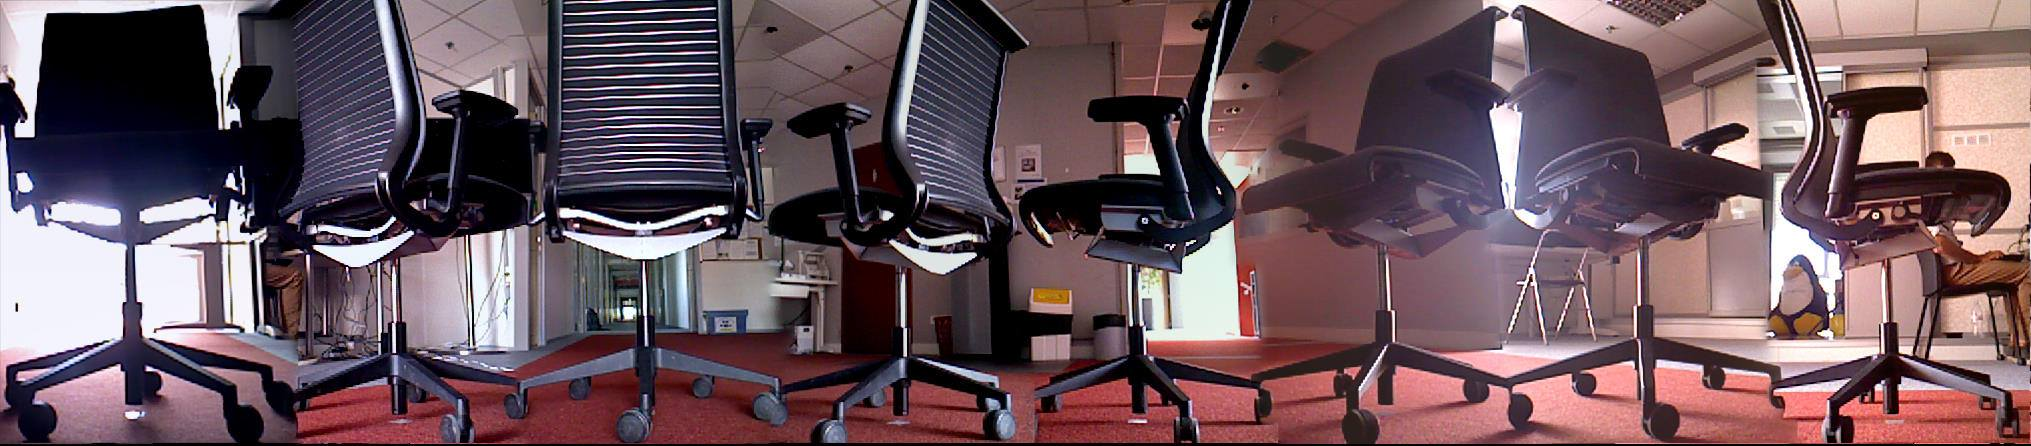
\includegraphics[width=\textwidth]{chair_db.jpg}}		
\end{figure}

Une première évaluation proposée consiste à faire un tour complèt autour de l'objet à être reconnu en quatre positions angulaires différentes : $0, 45, 90$ et une dernière choisi de manière aléatoire pour chaque objet. Le robot fait le tour à une vitesse de $0.35 \pm 0.1 m/s$ à une distance de $1.5m$, en enregistrant des images à $1hz$, ansi, une expérience typique consiste d'environ $25$  images d'angle différent et prendre $25 \pm 3$ seconds. Ensuite, trois différentes ratios sont calculés pour exprimer la reconnaissance d'objets, la reconnaissance de vue et la suivi des reconnaissances par la chaîne de Markov cachée.

{\color{green}
Dans le premier tableaux on retrouve le résultats de la reconnaissance donné par la comparaison des histogrammes provenant du *plus proche voisin*. Ce résultat estime la capacité de distinguer deux objets quelconques, en autre mots, cette capacité viens de la représentativité des descripteurs utilisés et l'efficacité de la mesure de similarité entre histogrammes.
}
